\section{MDP Formulation and Environment Implementation}
\label{sec:mdp}

\subsection{Problem Statement and Justification for Reinforcement Learning}
\label{subsec:mdp_justification}

In Workshop~1, movie recommendation on the MovieLens~32M dataset~\cite{harper2015movielens} was treated as a static supervised learning problem in which a regularized matrix factorization model (FunkSVD)~\cite{koren2009matrix} predicted pointwise ratings $\hat{r}_{u,i} = \mu + b_u + b_i + \mathbf{p}_u^\top \mathbf{q}_i$ and generated a fixed top-$K$ ranking for each user $u$. While effective for offline rating regression ($\text{RMSE} = 0.8041$), static supervised scoring violates three operational realities of interactive media platforms~\cite{afsar2022reinforcement}. First, user preferences within a browsing session are sequential and context-dependent: each recommendation presented to the user alters their immediate satisfaction state, shapes their short-term appetite for similar or contrasting genres, and constrains the remaining unvisited catalog. Second, supervised learning optimizes one-step pointwise error on historical observations without accounting for how an early recommendation influences subsequent engagement or the risk of session abandonment when a user encounters repeated uninteresting suggestions~\cite{zhao2018recommendations}. Third, because $54.8\%$ of all ratings in MovieLens~32M are concentrated in the top $1\%$ of titles, myopic supervised rankings over-exploit popular blockbusters and restrict catalog coverage to $8.00\%$.

Formulating sequential movie recommendation as a Markov Decision Process (MDP)~\cite{sutton2018reinforcement} directly resolves these structural limitations. In the RL paradigm, an autonomous recommendation agent interacts with a user over a multi-step session horizon $t \in \{0, 1, \dots, T-1\}$, sequentially selecting candidate films to maximize expected discounted cumulative return. Through explicit state transitions driven by immediate user feedback, the agent dynamically shifts its latent session belief toward accepted themes and away from rejected ones~\cite{zhao2018recommendations}. Furthermore, by incorporating self-information catalog novelty and genre diversity into the reward structure alongside relevance, the RL agent learns a long-horizon policy that balances the exploitation of high-affinity latent preferences with strategic exploration of under-exposed long-tail titles.

\begin{figure}[t]
\centering
\resizebox{\columnwidth}{!}{%
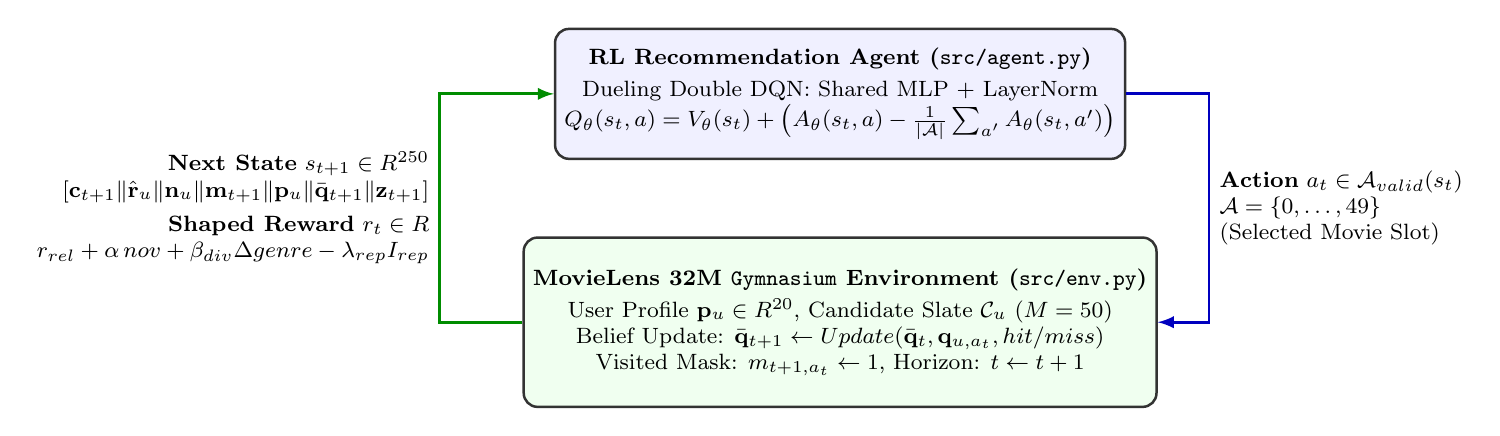
\begin{tikzpicture}[>=latex, font=\footnotesize]
    % Agent Box
    \node[draw=black!80, line width=0.9pt, rounded corners=5pt, fill=blue!6, minimum width=6.6cm, minimum height=1.65cm, align=center] (agent) at (0, 2.2) {
        \textbf{RL Recommendation Agent (\texttt{src/agent.py})}\\[2pt]
        Dueling Double DQN: Shared MLP + LayerNorm\\
        $Q_\theta(s_t, a) = V_\theta(s_t) + \bigl(A_\theta(s_t, a) - \frac{1}{|\mathcal{A}|}\sum_{a'} A_\theta(s_t, a')\bigr)$
    };

    % Environment Box
    \node[draw=black!80, line width=0.9pt, rounded corners=5pt, fill=green!6, minimum width=6.6cm, minimum height=2.15cm, align=center] (env) at (0, -0.7) {
        \textbf{MovieLens 32M \texttt{Gymnasium} Environment (\texttt{src/env.py})}\\[2pt]
        User Profile $\mathbf{p}_u \in \mathbb{R}^{20}$, Candidate Slate $\mathcal{C}_u$ ($M=50$)\\
        Belief Update: $\bar{\mathbf{q}}_{t+1} \leftarrow \text{Update}(\bar{\mathbf{q}}_t, \mathbf{q}_{u,a_t}, \text{hit/miss})$\\
        Visited Mask: $m_{t+1,a_t} \leftarrow 1$, Horizon: $t \leftarrow t+1$
    };

    % Action Arrow (Right side: Agent -> Env)
    \draw[->, line width=1.0pt, draw=blue!75!black] (agent.east) -- ++(1.05, 0) |- (env.east)
        node[pos=0.25, right, align=left, text=black] {
            \textbf{Action} $a_t \in \mathcal{A}_{\text{valid}}(s_t)$\\
            $\mathcal{A} = \{0, \dots, 49\}$\\
            (Selected Movie Slot)
        };

    % State & Reward Arrows (Left side: Env -> Agent)
    \draw[->, line width=1.0pt, draw=green!55!black] (env.west) -- ++(-1.05, 0) |- (agent.west)
        node[pos=0.25, left, align=right, text=black] {
            \textbf{Next State} $s_{t+1} \in \mathbb{R}^{250}$\\
            $[\mathbf{c}_{t+1} \| \hat{\mathbf{r}}_u \| \mathbf{n}_u \| \mathbf{m}_{t+1} \| \mathbf{p}_u \| \bar{\mathbf{q}}_{t+1} \| \mathbf{z}_{t+1}]$\\[3pt]
            \textbf{Shaped Reward} $r_t \in \mathbb{R}$\\
            $r_{\text{rel}} + \alpha\,\text{nov} + \beta_{\text{div}}\Delta\text{genre} - \lambda_{\text{rep}}\mathbb{I}_{\text{rep}}$
        };
\end{tikzpicture}%
}
\caption{Closed-loop Markov Decision Process interaction between the Dueling Double DQN recommendation agent and the MovieLens~32M \texttt{Gymnasium} simulator over a sequential user session.}
\label{fig:mdp_loop}
\end{figure}

\subsection{Formal Markov Decision Process $(\mathcal{S}, \mathcal{A}, \mathcal{P}, \mathcal{R}, \gamma)$}
\label{subsec:formal_mdp}

We model sequential movie recommendation as a finite-horizon discounted Markov Decision Process defined by the five-tuple $(\mathcal{S}, \mathcal{A}, \mathcal{P}, \mathcal{R}, \gamma)$, whose closed-loop interaction architecture is illustrated in Figure~\ref{fig:mdp_loop}. For each episode, an active user $u$ is sampled from the evaluation cohort along with a personalized candidate slate $\mathcal{C}_u = \{i_{u,0}, i_{u,1}, \dots, i_{u,M-1}\}$ of $M = 50$ movies. Each candidate $a \in \{0, \dots, 49\}$ is associated with its frozen Workshop~1 $L_2$-normalized FunkSVD latent embedding $\mathbf{q}_{u,a} \in \mathbb{R}^{20}$, normalized static predicted score $\hat{r}_{u,a} \in \mathbb{R}$, normalized self-information novelty $n_{u,a} \in [0, 1]$, and binary genre indicator vector $\mathbf{g}_{u,a} \in \{0, 1\}^{G}$.

\textbf{State Space ($\mathcal{S} \subset \mathbb{R}^{250}$).} At discrete decision step $t$, the environment exposes a continuous $250$-dimensional observation vector $s_t \in \mathcal{S} \subset \mathbb{R}^{250}$ constructed by concatenating seven semantically structured feature blocks:
\begin{equation}
\label{eq:state_vector}
s_t = \Bigl[\, \mathbf{c}_t^\top \;\Big\|\; \hat{\mathbf{r}}_u^\top \;\Big\|\; \mathbf{n}_u^\top \;\Big\|\; \mathbf{m}_t^\top \;\Big\|\; \mathbf{p}_u^\top \;\Big\|\; \bar{\mathbf{q}}_t^\top \;\Big\|\; \mathbf{z}_t^\top \,\Bigr]^\top \in \mathbb{R}^{250}.
\end{equation}
The first block $\mathbf{c}_t \in [-1, 1]^{50}$ encodes the dynamic session-item cosine similarities between the evolving unit-norm session preference vector $\bar{\mathbf{q}}_t \in \mathbb{R}^{20}$ and each candidate movie embedding $\mathbf{q}_{u,a} \in \mathbb{R}^{20}$, defined component-wise as $c_{t,a} = \text{sim}(\bar{\mathbf{q}}_t, \mathbf{q}_{u,a}) = \bar{\mathbf{q}}_t^\top \mathbf{q}_{u,a}$. The second block $\hat{\mathbf{r}}_u \in \mathbb{R}^{50}$ provides the static FunkSVD normalized affinity scores $\hat{r}_{u,a}$ derived from Workshop~1, anchoring the state in historical collaborative filtering estimates. The third block $\mathbf{n}_u \in [0, 1]^{50}$ contains the candidate self-information novelty values $n_{u,a} = -\log_2 P(i_{u,a}) / Z_{\text{nov}}$, where $P(i) = |\mathcal{R}_i^{\text{train}}| / |\mathcal{D}_{\text{train}}|$ is the empirical training interaction probability and $Z_{\text{nov}}$ is the catalog normalization constant, explicitly informing the agent of long-tail discovery potential. The fourth block $\mathbf{m}_t \in \{0, 1\}^{50}$ is the binary visited mask, where $m_{t,a} = 1$ indicates that candidate slot $a$ has already been recommended during steps $0, \dots, t-1$, and $m_{t,a} = 0$ otherwise. The fifth block $\mathbf{p}_u \in \mathbb{R}^{20}$ is the normalized static long-term user latent vector learned via FunkSVD, while the sixth block $\bar{\mathbf{q}}_t \in \mathbb{R}^{20}$ is the dynamic intra-session preference vector tracking the user's real-time taste trajectory. Finally, the seventh block $\mathbf{z}_t \in \mathbb{R}^{10}$ aggregates ten scalar session summary statistics: normalized step progress $t/T$, running session hit rate, immediate previous reward $r_{t-1}$, normalized consecutive miss streak ($\text{consecutive\_misses}/5$), mean session novelty accumulated so far, cumulative genre coverage ratio, clipped user rating bias $b_u$, normalized remaining horizon $(T-t)/T$, maximum cosine similarity among unvisited candidates $\max_{a : m_{t,a}=0} c_{t,a}$, and mean FunkSVD score among unvisited candidates. Together, these seven blocks satisfy $50 + 50 + 50 + 50 + 20 + 20 + 10 = 250$ dimensions and ensure the Markov property $\mathcal{P}(s_{t+1} \mid s_t, a_t, \dots, s_0, a_0) = \mathcal{P}(s_{t+1} \mid s_t, a_t)$.

\textbf{Action Space ($\mathcal{A} = \{0, 1, \dots, 49\}$).} The action space is discrete and consists of $M = 50$ candidate indices per user, $\mathcal{A} = \{0, 1, \dots, 49\}$. To construct a balanced yet tractable candidate pool $\mathcal{C}_u$ for user $u$ without leaked future information, the environment combines held-out interaction candidates from the evaluation split with high-affinity unseen candidates ranked by Workshop~1 FunkSVD scores, popular distractors, and high-novelty long-tail niche items, ordering the $50$ slots deterministically by baseline SVD affinity. At step $t$, the subset of admissible actions is defined by the unvisited candidate indices $\mathcal{A}_{\text{valid}}(s_t) = \{a \in \mathcal{A} : m_{t,a} = 0\}$, which shrinks by one slot per step under valid action masking.

\textbf{Transition Dynamics ($\mathcal{P}$).} The environment dynamics combine stochastic user instantiation at episode initialization with deterministic intra-episode state transitions conditioned on the user's response. When \texttt{reset()} is invoked, a user $u$ is sampled stochastically from the active partition ($\mathcal{D}_{\text{train}}$, $\mathcal{D}_{\text{val}}$, or $\mathcal{D}_{\text{test}}$), the visited mask is initialized to $\mathbf{m}_0 = \mathbf{0}_{50}$, the step counter is set to $t = 0$, and the initial session preference vector $\bar{\mathbf{q}}_0$ is initialized as a unit-normalized combination of the user's static factor $\mathbf{p}_u$, session target centroid $\bar{\mathbf{q}}_u^*$, and zero-mean Gaussian exploration noise $\boldsymbol{\xi} \sim \mathcal{N}(\mathbf{0}, 0.08^2 \mathbf{I})$. Given action $a_t \in \mathcal{A}$ at step $t$, let $h_t \in \{0, 1\}$ denote whether recommendation $i_{u,a_t}$ produces a positive user engagement (``hit'', $h_t = 1$) or a dissatisfaction/rejection event (``miss'', $h_t = 0$). For a valid unvisited action ($m_{t,a_t} = 0$), the dynamic session preference vector $\bar{\mathbf{q}}_{t+1}$ updates deterministically via signed latent momentum toward $\mathbf{q}_{u,a_t}$ on a hit and away from $\mathbf{q}_{u,a_t}$ on a miss:
\begin{equation}
\label{eq:session_belief_update}
\tilde{\mathbf{q}}_{t+1} = 
\begin{cases}
0.50\,\bar{\mathbf{q}}_t + 0.30\,\mathbf{q}_{u,a_t} + 0.20\,\bar{\mathbf{q}}_u^*, & \text{if } h_t = 1 \text{ (hit)}, \\[4pt]
0.75\,\bar{\mathbf{q}}_t - 0.20\,\mathbf{q}_{u,a_t} + 0.15\,\bar{\mathbf{q}}_u^*, & \text{if } h_t = 0 \text{ (miss)},
\end{cases}
\end{equation}
followed by unit $L_2$ normalization $\bar{\mathbf{q}}_{t+1} = \tilde{\mathbf{q}}_{t+1} / (\|\tilde{\mathbf{q}}_{t+1}\|_2 + \epsilon)$. Simultaneously, the visited mask updates via $m_{t+1,a} = m_{t,a} \lor \mathbb{I}[a = a_t]$, recomputing the dynamic similarity block $\mathbf{c}_{t+1}$ and summary statistics $\mathbf{z}_{t+1}$, and advancing the discrete clock $t \leftarrow t + 1$.

\textbf{Reward Function ($\mathcal{R}$) and Reward Shaping.} Because explicit ratings in MovieLens~32M exhibit $99.81\%$ catalog sparsity, a naive reward function that assigns non-zero feedback exclusively to observed historical pairs $(u, i)$ yields a degenerate sparse-reward signal that stalls temporal-difference learning and reinforces historical popularity bias. To provide an informative, well-calibrated learning signal at every step $t$, we design a composite shaped reward function combining relevance, catalog novelty, genre diversity, and repetition penalties:
\begin{equation}
\label{eq:composite_reward}
\begin{aligned}
r_t &= \mathbb{I}[m_{t,a_t} = 0] \Bigl( r_{\text{rel}}(u, a_t) + \alpha \cdot \text{nov}(u, a_t) \\
    &\quad + \beta_{\text{div}} \cdot \Delta\text{genre}(a_t) \Bigr) - \lambda_{\text{rep}}\,\mathbb{I}[m_{t,a_t} = 1].
\end{aligned}
\end{equation}
Here, the relevance component $r_{\text{rel}}(u, a_t)$ rewards positive user engagement ($h_t = 1$, where $r_{u,i} \ge 4.0$ or high latent session affinity) with a rating-scaled bonus and penalizes misses ($h_t = 0$):
\begin{equation}
\label{eq:relevance_reward}
r_{\text{rel}}(u, a_t) = 
\begin{cases}
1.0 + 0.25\,(r_{u,i} - 4.0), & \text{if } h_t = 1, \\[4pt]
-0.4, & \text{if } h_t = 0.
\end{cases}
\end{equation}
The second term in~\eqref{eq:composite_reward}, $\alpha \cdot \text{nov}(u, a_t)$ with weight $\alpha = 0.20$, rewards the agent for surfacing high-information, long-tail titles ($n_{u,a_t} \in [0, 1]$), directly counteracting the popularity bias quantified in Workshop~1. The third term, $\beta_{\text{div}} \cdot \Delta\text{genre}(a_t)$ with $\beta_{\text{div}} = 0.10$, grants a proportional bonus $\Delta\text{genre}(a_t) \in [0, 1]$ for covering film genres not yet represented in the current session slate, encouraging topical breadth. The fourth term applies a strict penalty $\lambda_{\text{rep}} = 1.5$ ($r_t = -1.5$) whenever an unmasked agent selects an already-visited slot ($m_{t,a_t} = 1$). Future rewards are discounted by $\gamma \in [0.90, 0.99]$ (with default $\gamma = 0.95$) to prioritize sustained multi-step user satisfaction over myopic one-step gains.

\textbf{Episode Termination.} An episode terminates when either of two conditions is met, corresponding to standard \texttt{Gymnasium} \texttt{truncated} and \texttt{terminated} flags~\cite{towers2024gymnasium}. First, an episode reaches natural horizon truncation (\texttt{truncated = True}) when the session completes $T = 10$ recommendation steps ($t = T$, with $T = 20$ also supported for extended-slate evaluation). Second, to model realistic user impatience and session churn, the environment triggers early termination (\texttt{terminated = True}, ``user abandonment'') if the agent suffers five consecutive misses ($\text{consecutive\_misses} \ge 5$), forfeiting all potential positive returns from the remainder of the session horizon.

\subsection{Gymnasium Simulator Design (\texttt{src/env.py})}
\label{subsec:gym_impl}

We implement the sequential movie recommendation simulator in \texttt{src/env.py} by subclassing \texttt{gymnasium.Env}~\cite{towers2024gymnasium} in Python. The class \texttt{MovieLensRecEnv} defines a discrete action space \texttt{spaces.Discrete(50)} corresponding to $\mathcal{A} = \{0, \dots, 49\}$ and a continuous box observation space \texttt{spaces.Box(low=-5.0, high=5.0, shape=(250,), dtype=np.float32)} matching $\mathcal{S} \subset \mathbb{R}^{250}$. All precomputed Workshop~1 FunkSVD factor matrices ($\mathbf{P} \in \mathbb{R}^{14998 \times 20}$, $\mathbf{Q} \in \mathbb{R}^{11589 \times 20}$), bias vectors, candidate pools, and novelty vectors are stored in contiguous 32-bit NumPy arrays so that state assembly and vector-matrix dot products execute in sub-millisecond time per step without dynamic memory allocation bottlenecks.

The environment implements the complete \texttt{Gymnasium} lifecycle API. Calling \texttt{reset(seed, options)} seeds the internal random number generator, selects a user episode from the active data split, initializes the session belief $\bar{\mathbf{q}}_0$ and visited mask $\mathbf{m}_0$, and returns the initial tuple \texttt{(obs, info)} containing the $250$-dimensional state vector and the valid action mask \texttt{info[\textquotesingle valid\_mask\textquotesingle]}. Calling \texttt{step(action)} executes the transition equations~\eqref{eq:session_belief_update}--\eqref{eq:relevance_reward}, updates session hit, novelty, and genre trackers, evaluates the horizon and abandonment conditions, and returns the standard five-tuple \texttt{(obs, reward, terminated, truncated, info)}. In addition, \texttt{MovieLensRecEnv} provides a human-readable \texttt{render()} method that formats a step-by-step session transcript displaying the active user index, step counter, recommended movie title and genres, hit/miss status, ground-truth rating, novelty in bits, and cumulative episode return.

Prior to neural network training, we validated the mathematical and software integrity of \texttt{MovieLensRecEnv} by executing $100$ diagnostic episodes under a uniform random policy ($\pi_{\text{rand}}$), following the verification protocol required for RL environments~\cite{raffin2021stable}. As presented in Section~IV (Figure~2 and Table~I), these $100$ random-policy episodes confirm that all $50$ discrete actions are sampled evenly across the action space without index-bias artifacts, that early abandonment (\texttt{consecutive\_misses >= 5}) and horizon truncation ($T=10$) behave exactly as specified, and that episode returns remain bounded and finite with zero \texttt{NaN} or out-of-bounds state transitions.
